\section{Modèle de processeur}

Cette partie vise à présenter les modifications du processeur afin d'assembler un système complet avec les blocs \gls{RAM}.
Pour tester la mémoire réalisée dans la partie précédente, le sujet fourni imagine un modèle de processeur élémentaire.
Cela permet à la fois de contextualiser le mini-projet tout en faisant appel aux connaissances d'architecture des ordinateurs vue les années passées.
Un modèle de processeur appelé \texttt{simple proc} est donné aux étudiants sous forme d'un code \textit{Verilog}.
Il est composé d'une mémoire interne pour stocker les instructions et données, mais ne comporte aucune entrée sortie.
Il n'est donc pas synthétisable, mais uniquement simulable.
L'objectif est de faire les modifications nécessaires pour assurer la compatibilité avec les blocs \gls{RAM}.
Cela passe par l'ajout d'un certain nombre de signaux et par la modification de l'\gls{ISA}. \\
\gap

Comme indiqué dans l'introduction, le logiciel \textit{Verilator} a été utilisé pour la simulation.
Sa particularité est de transformer la description \textit{Verilog} en \textit{C++}.
Le testbench peut être écrit en \textit{C++} offrant ainsi une vue plus haut niveau appréciée pour le test.
Le projet est largement utilisé dans le monde académique comme dans l'industrie.
On peut ainsi voir RISC-V Foundation, Microchip, NXP, Intel parmi ses utilisateurs.


\subsection{Modification de l'architecture}
La première modification à apporter est l'ajout d'entrées/sorties au processeur.
Cela doit permettre la connexion avec le bloc quadram.
Comme une entité (entity) en VHDL, le mot clé \texttt{module} permet d'adopter une vue externe.
On ajoute alors deux entrées clock (clk) et reset (nRst) pour la synchronisation.
Nous disposons dès lors d'une horloge, les instructions non synthétisable \texttt{step} peuvent être retirées après avoir rendu synchrone le process principal. La ligne \textit{Verilog} suivante permet cela.
\begin{lstlisting}[style=vhdl]
    always @ (posedge clk)
\end{lstlisting}
Il a été choisi précédemment de dupliquer le bus de données selon le sens de communication pour ne pas gérer la complexité induite par la bidirectionalité. Deux tableaux de bits \texttt{datain}, \texttt{dataout} sont définis un en entrée et l'autre en sortie. Leur taille est passée en paramètre pour garantir la généricité. Finalement, le bus d'adresse en déclaré en sortie car, seul le processeur en a le contrôle. Sa taille est, elle aussi, variable.
Le signal \texttt{we} pour "write enable" est utile pour contrôler la \gls{RAM} est déclarée comme sortie.
\begin{figure}[h]
    \centering
    \includegraphics[width=0.5\linewidth]{entité_proc.png}
    \caption{Entité simple proc}
    \label{entity_proc}
\end{figure}

Après l'analyse RTL, la vue externe obtenue figure \ref{entity_proc} est bien celle attendue.
Tous les signaux définis sont présents. Les paramètres pour la longueur des bus de données et d'adresse sont respectivement 32 et 12 dans cet exemple. \\
\gap

La seconde modification est nécessaire en raison du changement de mémoire.
Le processeur est initialement conçu avec une mémoire interne.
La contrainte concernant l'usage d'une mémoire externe rend l'accès à la donnée impossible pour les opérations arithmétiques.
Pour palier à cela, la solution est l'ajout de registres tampons d'une longueur égale à celle du bus de données.
Leur politique de gestion est explicitement laissée libre dans le sujet.
Les choix effectués par les étudiants concepteurs ne concernent pas la déclaration des registres, mais plutôt l'\gls{ISA}.
C'est pourquoi cette question sera abordée dans la partie suivante. \\
\gap

Le signal reset est choisi comme étant actif à l'état bas, son activation a pour effet de mettre à zéro les registres PC, IR, SR, reg\_A, reg\_B et le signal we.

\subsection{Modification de l'ISA}
Une ISA est définie comme étant un modèle abstrait d'un ordinateur.
Elle spécifie les instructions, les registres, les types de données et les fondamentaux de la gestion mémoire.
L'ISA ne décrite pas l'architecture d'un \gls{CPU} mais sert à sa conception.
Elle garantit la compatibilité au niveau binaire de deux implémentations \cite{ISA_wiki}.
Dans notre cas, l'ISA n'est pas proprement définit, c'est à nous de l'adapter pour répondre au comportement demandé. \\
Précédemment, une solution a été implémentée pour palier à l'inaccessibilité des données par les instructions arithmétiques.
Elle consiste à ajouter deux registres tampons A et B.
Il existe différentes philosophies de processeur parmi elles les plus connues, \gls{RISC} et \gls{CISC}.
Elles sont différentes sur plusieurs points. 
Pour ce qui nous intéresse ici, les architecture \gls{RISC} sont plus simple et exécute les instructions en un seul coup d'horloge. Les processeurs \gls{CISC} sont plus complexes et disposent d'instructions plus puissantes. 
Étudions cela à travers l'addition. En x86 (\gls{CISC}), l'instruction \texttt{add <reg>,<mem>} peut prendre en opérande un registre et une adresse mémoire \cite{x86_asm}. 
En langage ARM assembleur, \texttt{add Rd, Rm} ne peut se faire qu'entre deux registres \cite{ARM_ASM}.
Il faudra donc charger (LDR) les deux valeurs dans des registres avant d'effectuer une addition.
Pour des questions de simplicité, mais aussi car l'architecture \gls{RISC} sont particulièrement intéressantes pour l'embarqué, comme le montre la popularité de ARM et RISC-V, nous choisirons la philosophie \gls{RISC}. \\
Il convient alors de modifier les instructions arithmétiques.
Elles accèderont seulement aux registres.
La règle générale est alors $A = A \quad o \quad B$ ou les lettres A et B représentent les registres et le symbole $o$ les opérations arithmétiques telles que l'addition, la soustraction et la multiplication. 
Le résultat du complément est également stocké dans A.
Le code \textit{Verilog} dans le cas de l'addition est le suivant :
\begin{lstlisting}[style=vhdl]
`ADD:
begin
    reg_A = reg_A + reg_B;
    setcondcode(reg_A);
end
\end{lstlisting}
L'appel à la fonction \texttt{setcondcode()} met à jour l'état du registre SR avec le résultat du calcul. \\
\gap

Dans l'état actuel du processeur, il n'est pas possible d'affecter une valeur aux registres A et B.
Pour palier à cela, deux instructions "load" sont ajoutées LDA et LDB.
Il existe une subtilité quant à leur mise en place. Contrairement à la mémoire interne, la RAM n'est pas accessible immédiatement.
D'abord l'adresse est placée sur son bus puis, au cycle suivant, la valeur de la case mémoire est placée sur le bus de données.
Cela écarte une solution naïve qui viserait à écrire l'adresse et récolter la donnée de manière synchrone au premier front.
Il faudrait plutôt affecter la valeur au registre au front d'horloge suivant.
Nous avons choisi, en nous basant sur le processeur précédemment étudié le Z80, d'utiliser un signal \texttt{t\_wait}.
Il permet d'ajouter un cycle horloge au cycle machine qui était initialement systématiquement égaux.
Lorsque \texttt{t\_wait} vaut 1, le registre \texttt{PC} n'est pas incrémenté, et \texttt{IR} maintenu à sa valeur précédente.
\begin{figure}[h]
    \centering
    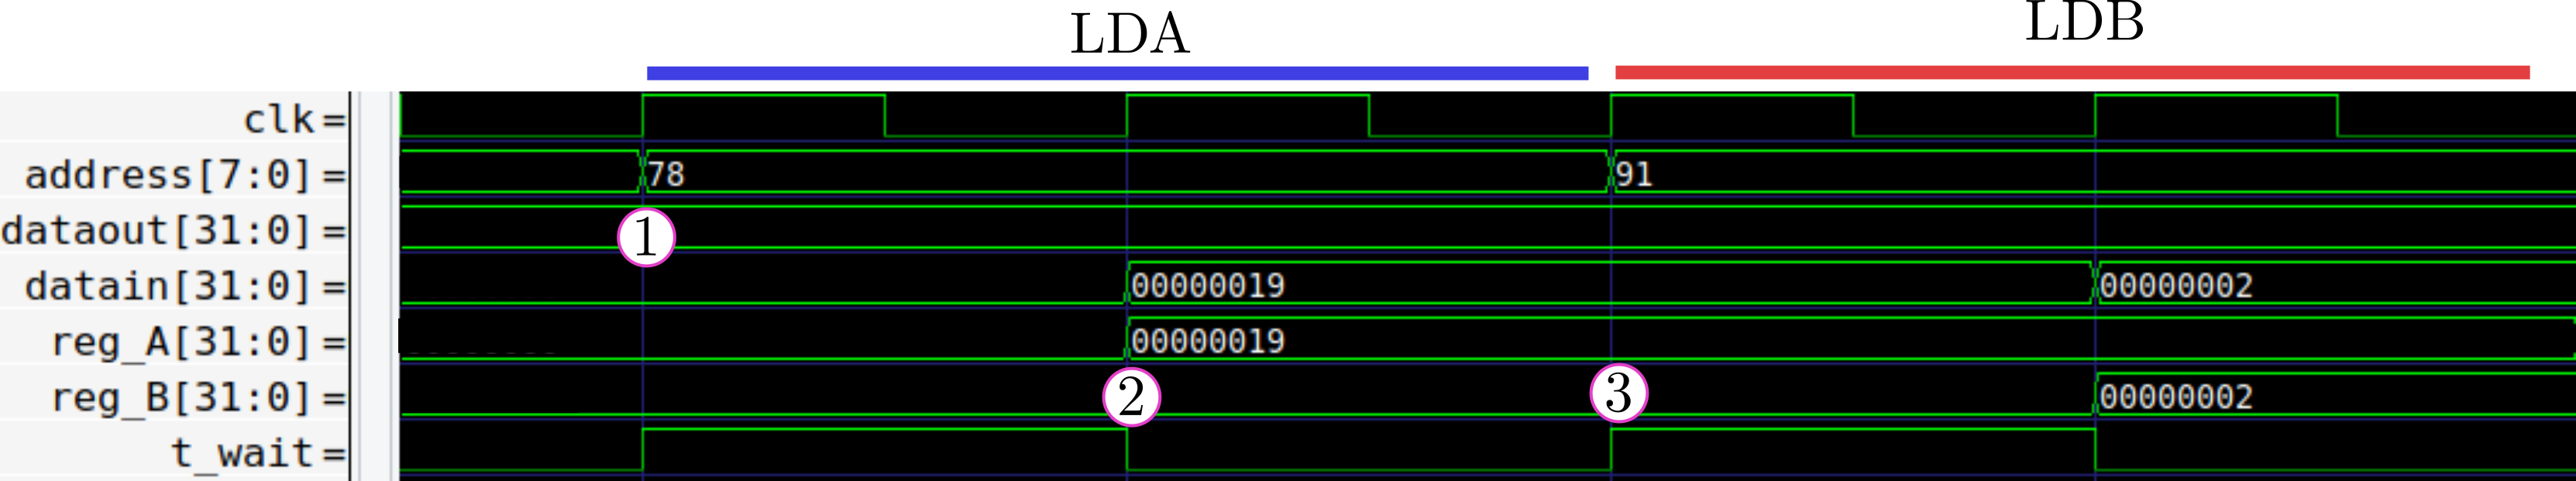
\includegraphics[width=\linewidth]{validation_twait.draw.png}
    \caption{Chronogramme test LDA et LDB avec \texttt{t\_wait}}
    \label{fig:test_LD}
\end{figure}
Le chronogramme commenté figure \ref{fig:test_LD} présente les résultats obtenus après simulation.
Un testbench permet de charger la mémoire avec les instructions \texttt{LDA 0x78} et \texttt{LDB 0x91}.
Il fournit ensuite une réponse semblable au comportement de la \gls{RAM} en plaçant au second front une valeur sur le bus de données.
A l'instant du label 1, l'instruction \texttt{LDA 0x78} est exécutée, 0x78 est placé sur le bus d'adresse et \texttt{t\_wait} passe à l'état haut.
Puis à l'instant 2, lors du second front, la donnée 0x19 est fournie et affectée au registre A.
Enfin, à l'instant 3, la valeur 0x19 est maintenue dans le registre.
L'instruction de chargement (load) a fonctionné.
Le même raisonnement s'applique pour \texttt{LDB}.
La solution présentée, visant à allonger les instructions de chargement d'un cycle, est simple à mettre en œuvre.
Elle a cependant le désavantage évident de multiplier par deux le temps d'exécution. \\
Cette stratégie peut être appliquée de la même façon à l'instruction de stockage (\texttt{STR}).
Le même signal \texttt{t\_wait} est mis à l'état haut afin de figer le processeur pendant un coup d'horloge.
Les bus conservent alors leur état et la mémoire peut assimiler la valeur.
On propose de présenter la validation par le résultat du testbench.
Dans le testbench en \textit{C++}, une structure est définie correspondant à chaque instruction.
La fine séparation fournie par les \textit{bit field} du langage C permet d'assigner une taille à chauqe champs.
\begin{lstlisting}[style=CStyle]
typedef struct {
    uint16_t BB : 12;
    uint16_t AA : 12;
    uint8_t RESERVED : 3;
    uint8_t IM : 1;
    uint8_t OPCODE : 4;
} _STR_t;
\end{lstlisting}
La ligne \texttt{STR.field.IM = 1;} ci-dessous, correspond ainsi à l'affectation d'un seul et unique bit à l'emplacement souhaité.
Cela facilite l'écriture et évite de passer par la notation binaire ou hexadécimale.
\begin{lstlisting}[style=CStyle]
STR.field.IM = 1;
STR.field.AA = 0xAF; /* idenfiable random data value */
STR.field.BB = 0x81; /* address */
dut->simple_proc__DOT__MEM[0] = STR.val; /* set memory */
\end{lstlisting}
La dernière ligne de l'extrait ci-dessus réalise l'initiation de la mémoire interne.
La première instruction, à l'index $[0]$ est donc un \texttt{STR}.
\begin{lstlisting}[style=CStyle]
/* assert STR test when IR reg == STR */
if (dut->simple_proc__DOT__IR == STR.val && dut->clk == 1){ 
    if ((dut->address == 0x81) && (dut->dataout == 0xAF)){
      printf("Success asserting STR test 1 \n");
    }
    else{
      printf("STR failed. Addr:%d data:%d \n", dut->address, dut->dataout);
    }
}
\end{lstlisting}
Le test pour vérifier la conformité de l'instruction s'attache à contrôler l'état du bus d'adresse et de donnée sachant l'instruction encodée.
Le résultat du terminal est alors :
\begin{lstlisting}[frame=single, basicstyle = \ttfamily \footnotesize]
    Success asserting STR test 1
\end{lstlisting}
Une seconde confirmation avec les chronogrammes est effectuée.
Elle confirme le premier diagnostique.\\

Un testbench en \textit{C++} est écrit pour chacune des instructions LDA, LDB, STR et ADD.
Cela peut paraitre redondant, mais on s'assure ainsi qu'une modification sur une instruction n'impacte pas les autres.
Nous sommes satisfaits d'avoir suivi cette méthode, car cela nous a gagné un temps précieux dans l'étape suivante combinant RAM et processeur.


%Nous n'avons pas réussi à définir le codage des instructions de manière générique dans le temps imparti.
